% Gemini theme
% https://github.com/anishathalye/gemini

\documentclass[final]{beamer}

% ====================
% Packages
% ====================

\usepackage[T1]{fontenc}
\usepackage{lmodern}
\usepackage[size=custom,width=121.92,height=91.44,scale=1.27]{beamerposter}
\usetheme{gemini}
\usecolortheme{gemini}
\usepackage{graphicx}
\usepackage{booktabs}
\usepackage{tikz}
\usetikzlibrary{shapes.geometric, arrows}
\usepackage{pgfplots}
\pgfplotsset{compat=1.14}
\usepackage[export]{adjustbox}
\usepackage{wrapfig}
\usepackage{booktabs}

%%%%%SCALING THE PDF%%%%%


% ====================
% Lengths
% ====================

% If you have N columns, choose \sepwidth and \colwidth such that
% (N+1)*\sepwidth + N*\colwidth = \paperwidth
\newlength{\sepwidth}
\newlength{\colwidth}
\setlength{\sepwidth}{0.025\paperwidth}
\setlength{\colwidth}{0.3\paperwidth}

\newcommand{\separatorcolumn}{\begin{column}{\sepwidth}\end{column}}

% ====================
% Title
% ====================

\title{Here Comes the Bloom: Investigating Freshwater Cyanobacteria Bloom and Non-Bloom Sites in Ontario}

\author{Alexander Turco \inst{1} \and George S. Long \inst{1,2} \and H.E. Schellhorn \inst{1} \and G. Brian Golding \inst{1}}

\institute[shortinst]{\inst{1} Department of Biology, McMaster University, Ontario, Canada  \and %
                      \inst{2} McMaster aDNA Centre, McMaster University, Ontario, Canada }
                      
% ====================
% Footer (optional)
% ====================
\footercontent{
  \href{www.macwater.org}{macwater.org} \hfill
  MacWater Challenges in Water Monitoring 2022 Hamilton, Ontario \hfill
  \href{mailto:turcoa1@mcmaster.ca}{turcoa1@mcmaster.ca}}
% (can be left out to remove footer)

% ====================
% Logo (optional)
% ====================

% use this to include logos on the left and/or right side of the header:
% \logoright{
\includegraphics[height=7cm]{logo1.pdf}}
 \logoleft{
\includegraphics[height=7cm]{logo1.png}}

% ====================
% Body
% ====================

\begin{document}

\begin{frame}[t]
\begin{columns}[t]
\separatorcolumn

\begin{column}{\colwidth}

  \begin{block}{Abstract}

    Reports of algal blooms are on the rise both globally and domestically, more specifically here in Ontario. 
    The number of blooms containing toxigenic cyanobacteria have been increasing, 
    which poses major threats to the environment, as well as human and animal populations. Many models
    for studying blooms are able to predict biomass concentrations of cyanobacteria in large bodies of water,
    but there are a lack of models which are able to describe the composition and toxicity of these blooms. 
    
    Due to an increasing demand for the genetic evaluation of microbes associated with blooms, as well as 
    the limitations involved with the culturing of cyanobacteria, a metagenomic approach was utilized in this study. 
    This allowed for a deeper understanding of the microbial diversity of algal blooms, and permitted
    the assembly of potentially toxin producing genomes.
    
    This study focuses on the composition of microbial communities in the collected
    samples along with the genomic assembly of four organisms found to play key roles in the development of harmful algal
    blooms. Overall, the findings reveal differences in cyanobacterial communities across bloom and non-bloom sites, as 
    well as strain level differences in the organisms which dominate blooms and potentially contribute to toxicity.
    
  \end{block}

  \begin{block}{Background}

    In collaboration with the Ministry of the Environment and Climate Change (MOECC), bloom and non-bloom sites
    were sampled from a variety of freshwater locations around Ontario in 2015 and sent for 16s rRNA sequencing 
    and shotgun metagenomic sequencing.
     
     \begin{table}[h]
	\centering
	\begin{tabular}{cccc}
	\toprule
	\textbf{Type of Sequencing} & \textbf{Bloom Samples} &\textbf{Non-Bloom Samples} & \textbf{Unknown Samples} \\
	\midrule
	16s rRNA & 16 & 4 & 36 \\ 
 	Shotgun & 12 & 16 & 0 \\ 
	\bottomrule
	\end{tabular}
      \end{table}
    
  \end{block}

  \begin{alertblock}{Workflow}
  \begin{figure}
    \centering

     \tikzstyle{startstop} = [rectangle, rounded corners, minimum width=3cm, minimum height=1cm,text centered, draw=black, fill=blue!30]
     \tikzstyle{begin} = [rectangle, rounded corners, minimum width=3cm, minimum height=1cm,text centered]
     \tikzstyle{arrow} = [ultra thick,line width=1mm,->,>=stealth]
   
   	\begin{tikzpicture}[node distance=2cm]
   	
	\node (start) [begin] {};
        \node (1) [startstop, right of=start, xshift=5cm]{Raw 16s rRNA Samples};
        \node (2) [startstop, left of=start, xshift=-5cm]{Raw Shotgun Samples};
        \node (4) [startstop, below of=start, yshift=-1cm]{\texttt{FastP}};
        \node (5) [startstop, right of=4, xshift=9cm]{Cleaned 16s Samples};
        \node (6) [startstop, left of=4, xshift=-10cm]{Cleaned Shotgun Samples};
        \node (7) [startstop, below of=5, yshift=-4cm]{\texttt{QIIME2}};
        \node (8) [startstop, below of=6, yshift=-3cm]{\texttt{BWA}};
        \node (10) [startstop, below of=8, yshift=-1cm, xshift=-4cm]{\texttt{SPAdes}};
        \node (11) [startstop, below of=8, yshift=-1cm, xshift=4cm]{Heterozygous SNPs};
        \node (12) [startstop, below of=10, yshift=-0.5cm]{\texttt{BLASTn}};
        \node (13) [startstop, below of=8, yshift=-5.5cm]{\texttt{Mashtree}};
        \node (14) [startstop, below of=5, yshift=-1cm]{\texttt{KRAKEN2}};
        \node (15) [startstop, below of=6, yshift=-0.5cm]{\texttt{KRAKEN2}};
        
        
        \draw [arrow] (1) -- (4);
        \draw [arrow] (2) -- (4);
        \draw [arrow] (4) -- (5);
        \draw [arrow] (4) -- (6);
        \draw [arrow] (6) -- (15);
        \draw [arrow] (5) -- (14);
        \draw [arrow] (8) -- (10);
        \draw [arrow] (8) -- (11);
        \draw [arrow] (10) -- (12);
        \draw [arrow] (12) -- (13);
        \draw [arrow] (14) -- (7);
        \draw [arrow] (15) -- (8);
        

   \end{tikzpicture}
   \end{figure}

  \end{alertblock}

\end{column}

\separatorcolumn

\begin{column}{\colwidth}

   \begin{block}{Phylogenetically Placing the Samples}
    
    \begin{figure}
    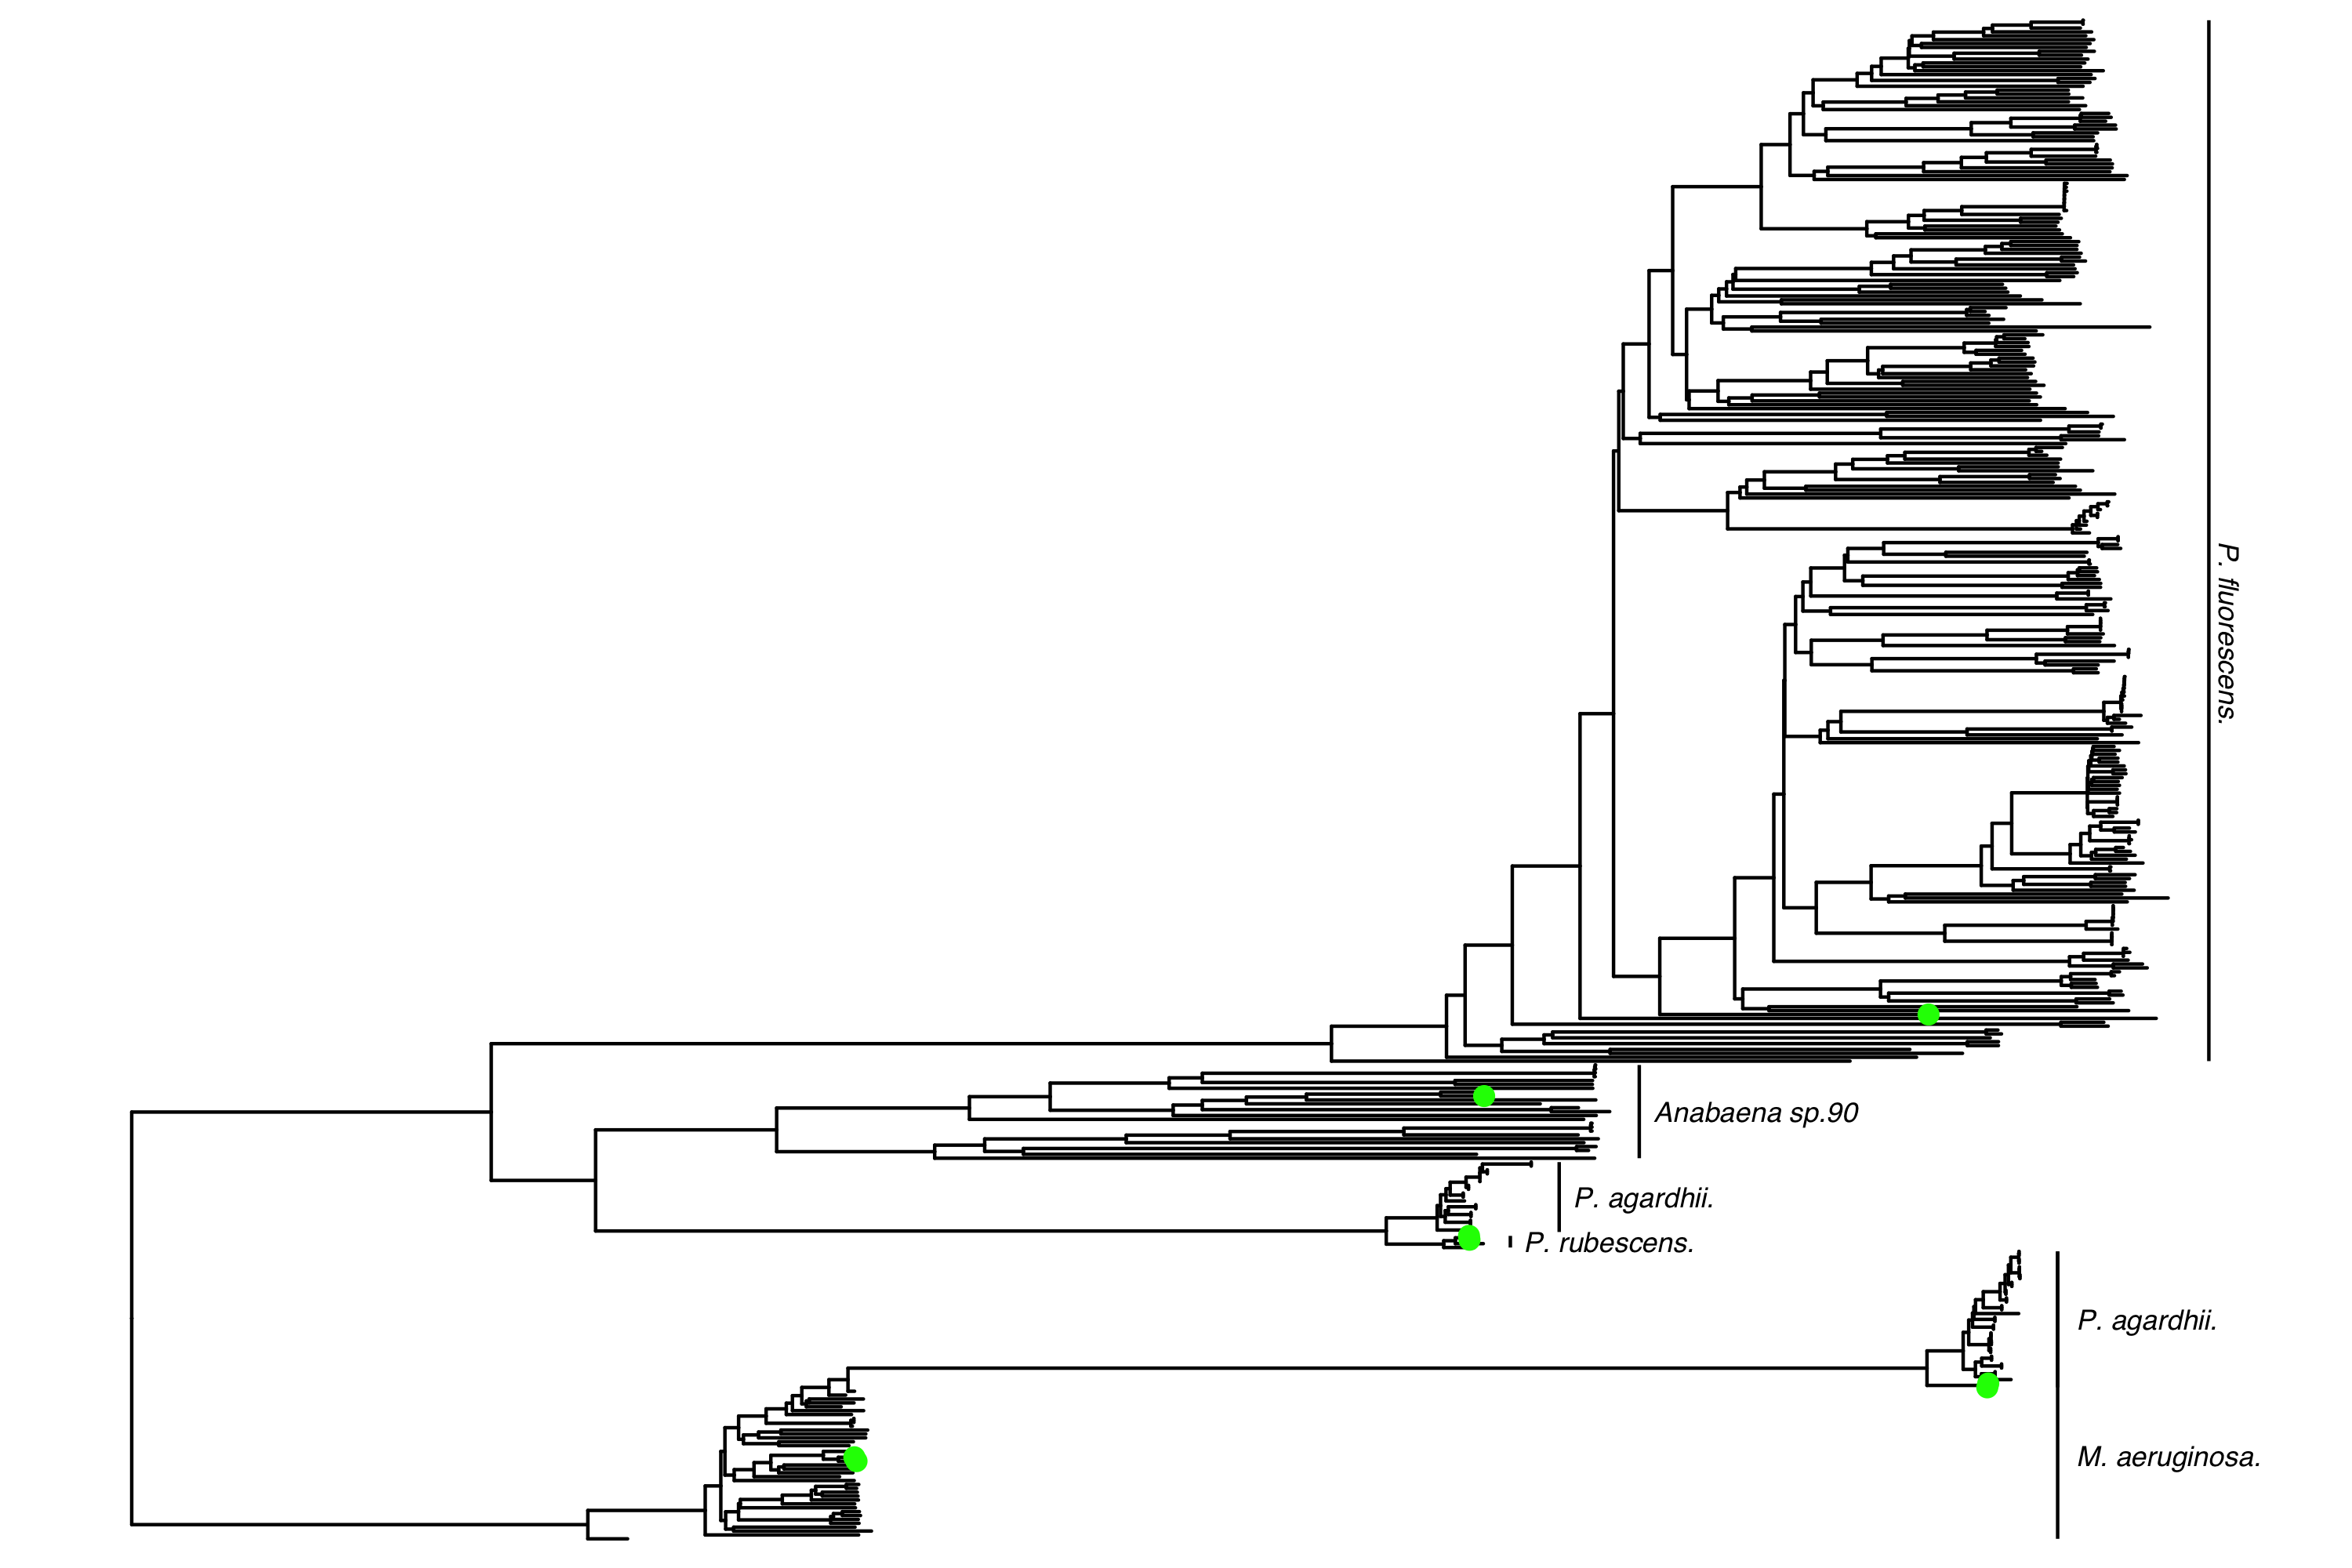
\includegraphics[width=\textwidth]{mashphylogeny.png}
     \caption{Mash Distance Phylogeny of five different species known to dominate algal blooms }
     \end{figure}
     
     Five different types of bacterial genomes were found to dominate in six bloom site shotgun samples. A Mash distance phylogeny was created
     which shows the blasted sample sequences among different strains of the same bacterial species collected from the NCBI database.
     The formation of unique clades is evident, and the blasted assemblies falling into the specific clades highlights the 
     unique species of \emph{Microcystis aeruginosa}, \emph{Planktothrix rubescens}, \emph{Planktothrix agardhii}, \emph{Anabaena sp.90}, and
     \emph{Pseudomonas aeruginosa} found in the samples.

  \end{block}

  \begin{block}{Multiple Strain Potential at Bloom Sites}
    
  \begin{figure}
    \noindent\begin{minipage}{0.3\textwidth}% adapt widths of minipages to your needs
    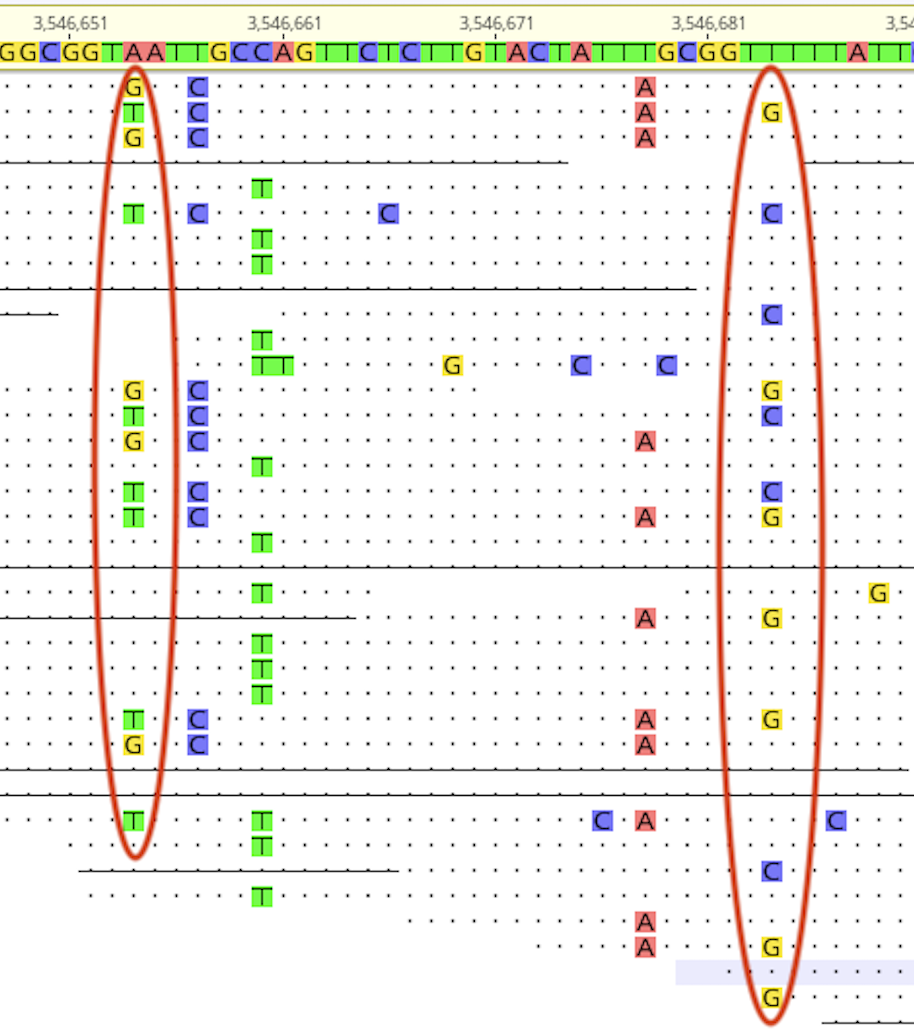
\includegraphics[width=\linewidth]{heterosnps.png}
    \end{minipage}%
    \hfill%
    \begin{minipage}{0.65\textwidth}\raggedright
    Of the five different types of bacterial genera explored in the samples, four contained potentially toxic, microcystin
    producing strains. Single nucleotide polymorphisms (SNPs) were examined in bloom samples which contained these
    organisms in order to determine if heterozygous SNPs were present. Heterozygous SNPs were present in all four samples,
    with the largest amount being found in a sample containing \emph{Microcystis aeruginosa}. These heterozygous SNPs provide potential evidence
    of different copies of the same gene and are therefore potentially indicative of multiple strains of \emph{Microcystis aeruginosa} 
    present at a single bloom site.
    \end{minipage}
    \caption{Showing two heterozygous SNP sites from a bloom sample containing \emph{Microcystis aeruginosa} }
   \end{figure}
  
  \end{block}

\end{column}

\separatorcolumn

\begin{column}{\colwidth}

  \begin{block}{Differences in Bacterial Composition of Bloom and Non-Bloom Sites}
  
  Amplicon sequencing analysis using Quantitative Insights Into Microbial Ecology (QIIME2) revealed different bacterial
  compositions of bloom, non-bloom, and unknown sites.
  
  \begin{enumerate}[$\Rightarrow$]
  \item At the phylum level, all types of samples tend to be dominated by proteobacteria, actinobacteria, and cyanobacteria.
  \item Larger relative abundance of cyanobacteria in bloom sites compared to non-bloom sites, suggesting a key role played by cyanobacteria in the formation of blooms.
  \item Larger relative abundance of verrucomicrobia in bloom sites compared to non-bloom sites.
  \end{enumerate}
  
   \begin{figure}
      \centering
      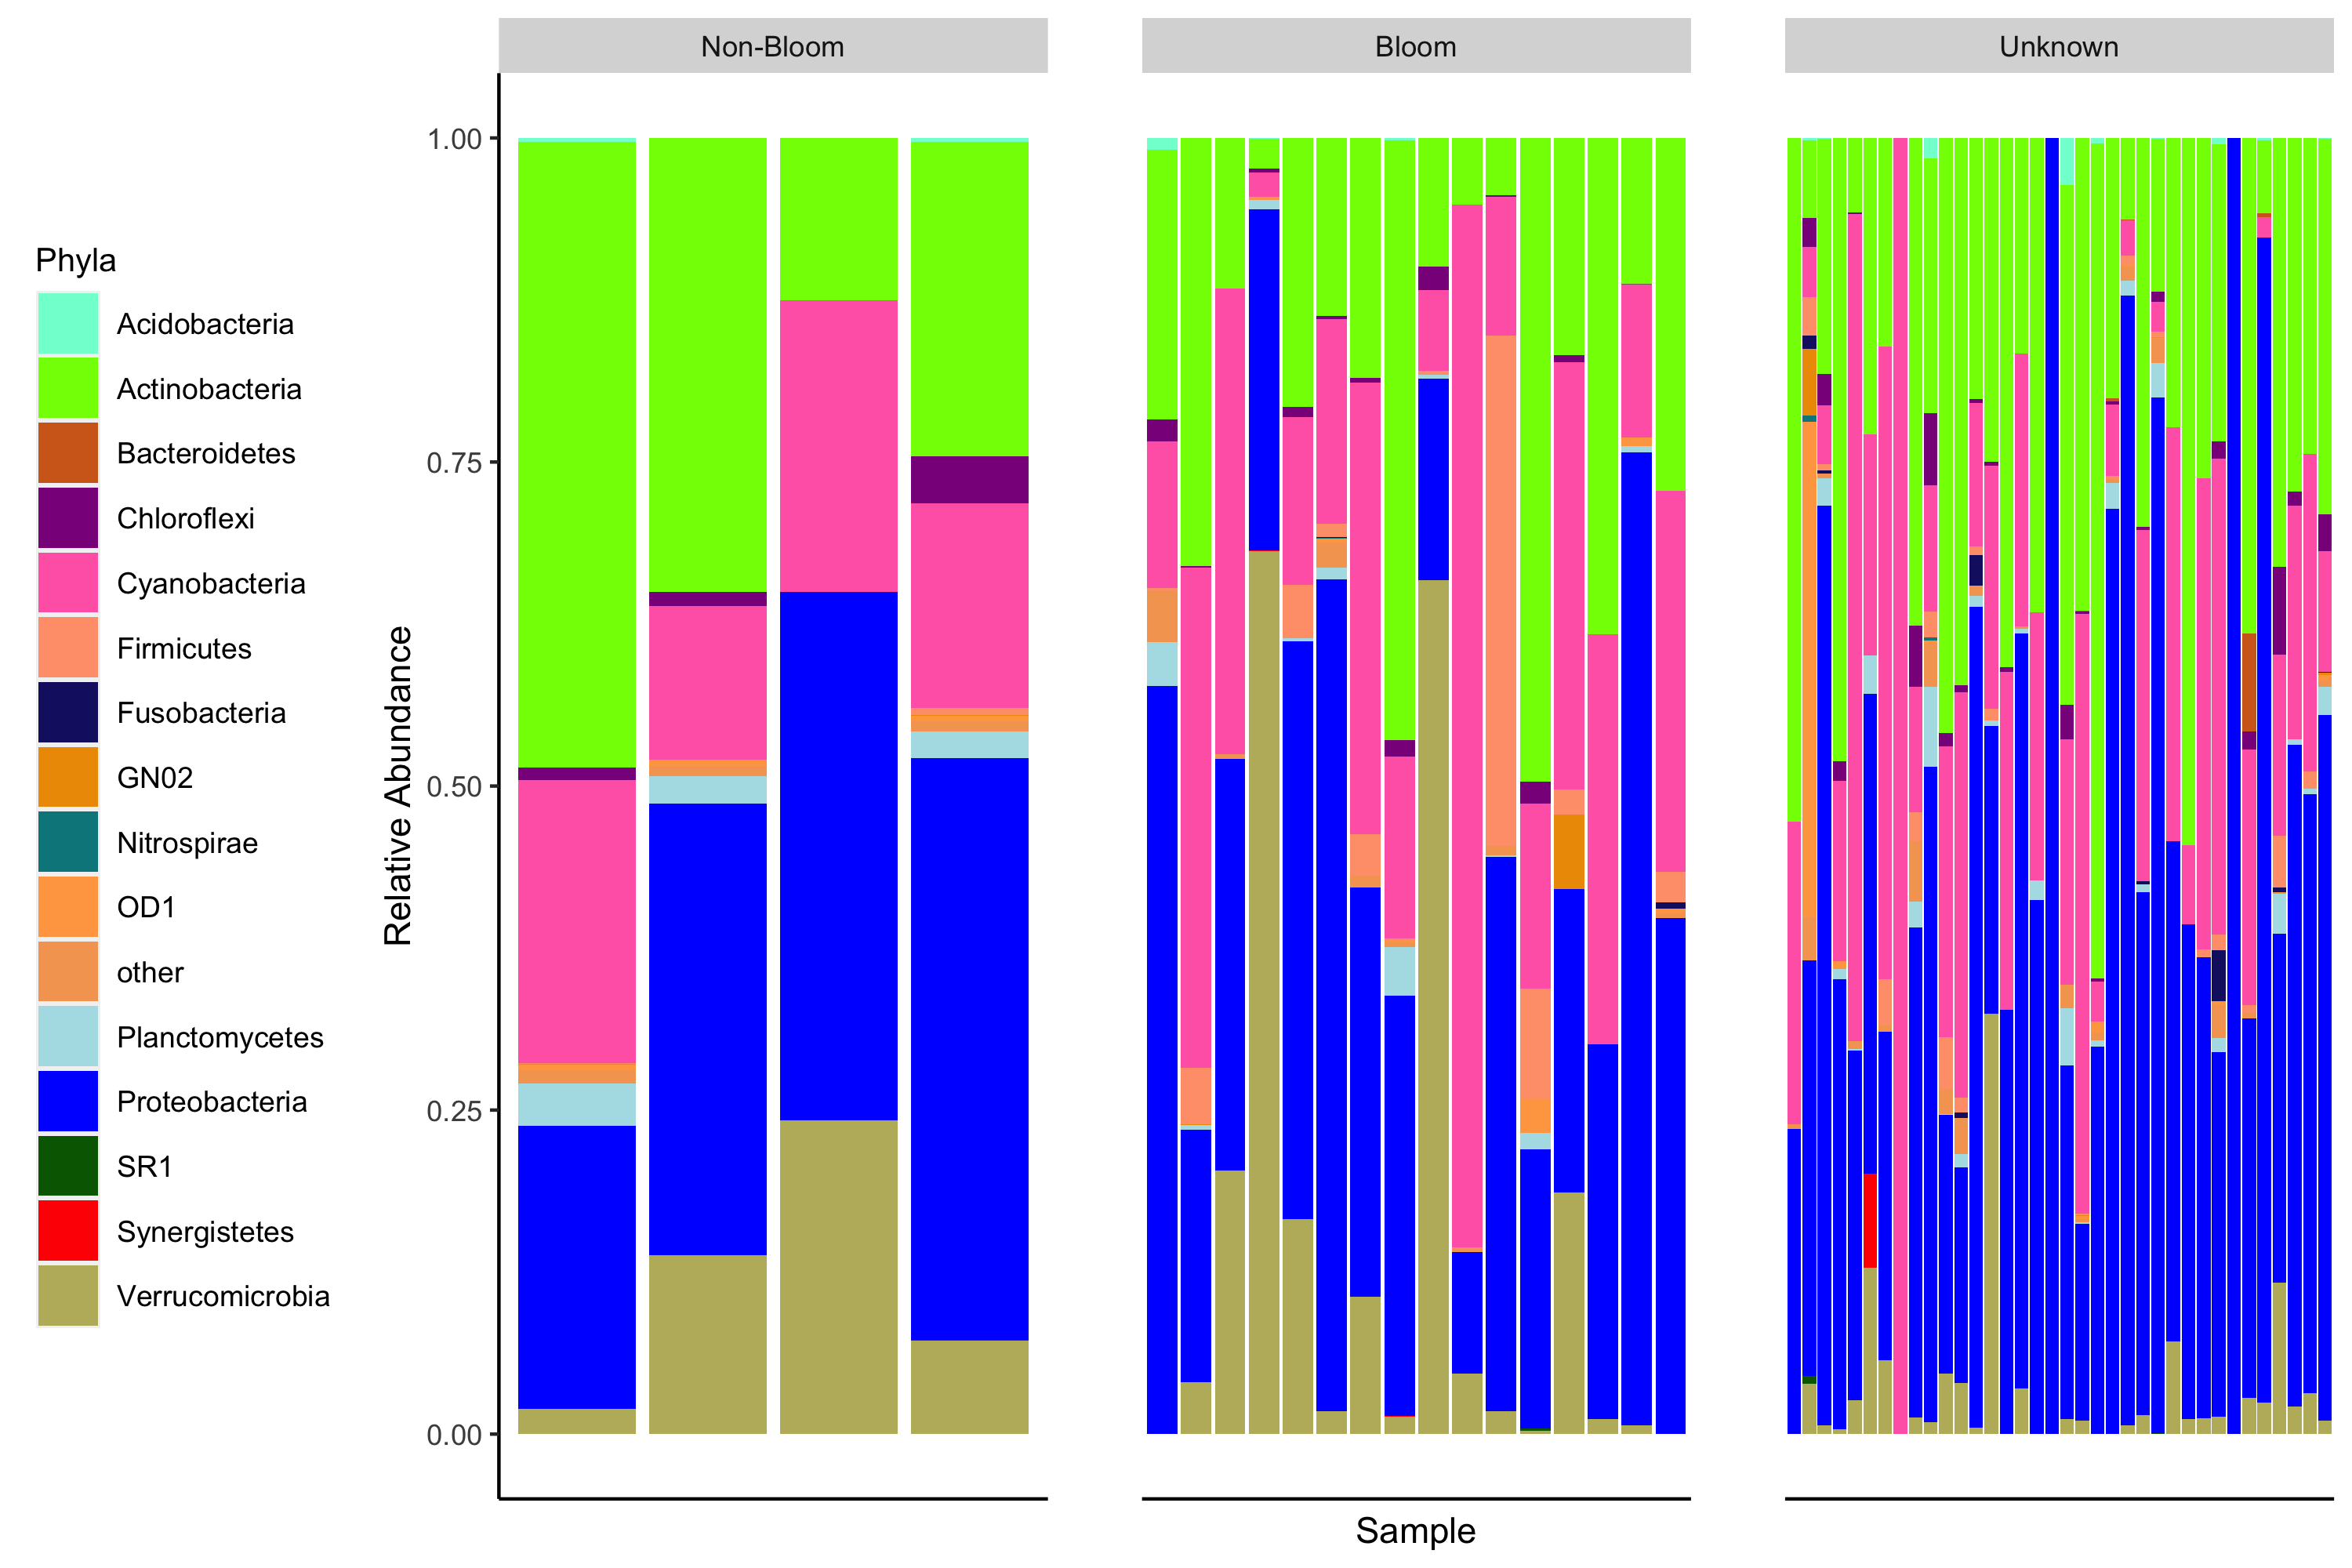
\includegraphics[width=\textwidth]{16s_phyla.png}
      \caption{Relative Abundance of 16s rRNA Microbial Community Phyla in Bloom, Non-Bloom, and Unknown Sites}
    \end{figure}

  \end{block}
  
  \begin{block}{Future Work}
  
   \begin{enumerate}[$\Rightarrow$]
  \item Uncovering gene level differences in the microcystin biosynthesis gene operon of toxic and non-toxic genera of cyanobacteria.
  \item Assessing the differences in composition of algal blooms based on factors such as location, time of year, and temperature.
  \item Identifying not only taxonomic differences, but also functional differences between bloom and non-bloom environments.
  \item Utilizing metagenomic approaches to characterize and monitor harmful algal blooms in combination with water quality and environmental data to better understand and predict the toxicity of blooms.
  \end{enumerate}
    
  \end{block}


  %\begin{block}{References}

    %\nocite{*}
    %\footnotesize{\bibliographystyle{plain}\bibliography{poster}}

  %\end{block}

\end{column}

\separatorcolumn
\end{columns}
\end{frame}

\end{document}
